\documentclass[14pt]{mmcs-article}
\usepackage[russian]{babel}
\usepackage{amsmath, amsthm, amsfonts, amssymb}

% После кванторов ставить отступ
% Починить \mod (\mathsc) -- сейчас там большой пробел в начале

% Надо бы настроить правильную сквозную нумерацию замечаний, теорем e.t.c

% Надо сделать примеры не в растре, а средствами теха

\graphicspath{{images/}}

\begin{document}

\section*{Введение}

\textbf{Определение 1.}

% Нужно написать определение с кратными дугами, а потом аккуратно попробовать упростить до варианта с парой вершин

\textsl{Двудольным графом} будем называть пару $\langle V,E \rangle$, такую, что:

\begin{itemize}
    \item $V = A \cup B$ и $A \cap B = \emptyset$ ;
    \item $e = \{a, b\}, a \in A, b \in B \forall e \in E$;
\end{itemize}

Где $V$ ~--- множество вершин, разбитое на два непересекающихся подмножества $A$ и $B$.
$E$ ~--- множество дуг. Дуга ~--- это упорядоченная пара вершин, называемых инцидентными этой дуге.

\textbf{Определение 2.}

% пример

% Надо потом аккуратно в замечении это всё дело переопределить так, чтобы запись была более компактная (отказаться от отображения, использовать пары)

% Что если задавать путь через последовательность вершин, а не дуг? -- к этому перейдём через замечание

% Как-то надо было единообразно заименовать пути: мю, эта
% фи и пси обычно отображения

%% Поменять местами определения. Начальную и коменчную вершины пути дать прямо тут, как его неотъемлемую часть

Пусть $G$ ~--- граф $G = \langle A \cup B, E \rangle$.
Упорядоченную последовательность дуг $\mu = (e_1, ..., e_d)$ будем называть путём, если у дуги $e_i$, где $i = 2, ..., d-1$, одна инцидентная вершина общая с дугой $e_{i-1}$, а другая ~--- общая с дугой $e_{i+1}$.

\textbf{Определение 3.}

% Вот это мне не нравится, кажется, мы от этого как-то избавлялись, но оно не сохранилось -- от этого избавились, давая начальную и конечную вершины в определении самого пути

Вершину дуги $e_1$, не являющаяся общей с дугой $e_2$, называют первой вершиной пути.

Вершину дуги $e_d$, не являющаяся общей с дугой $e_{d-1}$, называют последней вершиной пути.

\textbf{Определение 4.}

Циклом будем называть путь, у которого совпадают первая и последняя вершины.

\textbf{Определение 6.}

\textsl{Обхватом графа} называют длину его минимального цикла.

\textbf{Замечание 1.}

Отметим, что обхват любого двудольного графа является чётным числом, большим, чем два.

\textbf{Замечание 2.}

Известно, что на практике для кодирования эффективнее использовать графы с большим обхватом.

\textbf{Определение 5.}

% Характеристика дуги внутри пути (в какую сторону путь проходит дугу)

С каждым путём $\mu$ свяжем характеристическую функцию $\chi_\mu(e)$.
Так, если $v_0$ ~--- первая вершина пути, то
\[
    \chi_{\mu}(e_1) =
    \left\{
        \begin{array}{ll}
        1,  & v_0 \in A;\\
        -1, & v_0 \in B. \\
        \end{array}
    \right..
\]

$\forall i \in 2, ..., d$, если $e_1 = (a, b)$, то
\[
    \chi_{\mu}(e_i) =
    \left\{
        \begin{array}{ll}
        1,  & a \text{ инцидентна дуге } e_{i-1};\\
        -1, & \text{в противном случае}. \\
        \end{array}
    \right..
\]

\pagebreak
\section*{Метаграфы}

\textbf{Определение 6.}

\textsl{Метаграфом} будем называть тройку $\langle V,E,w \rangle$, такую, что:

\begin{itemize}
    \item $\langle V,E \rangle$ ~--- двудольный граф;
    \item $w: E \rightarrow \mathbb{Z}$ ~--- отображение задающее веса дуг.
\end{itemize}

На (рис. \ref{image:2}) представлен пример метаграфа с тремя вершинами и четырьмя дугами.

\begin{figure}[H]
    \centering
    \begin{picture}(150,200)
        \put(75,165){\thicklines{\circle*{5}}}
        \put(70,170){$c_1$}
    
        \put(35,35){\thicklines{\circle*{5}}}
        \put(30,20){$i_1$}
    
        \put(115,35){\thicklines{\circle*{5}}}
        \put(110,20){$i_2$}
    
        \bezier{300}(75,165)(10,100)(35,35)
        \put(5,100){$+1$}

        \bezier{300}(75,165)(56,100)(35,35)
        \put(56,80){$0$}
    
        \bezier{300}(75,165)(140,100)(115,35)
        \put(125,100){$-1$}

        \bezier{300}(75,165)(94,100)(115,35)
        \put(87,80){$0$}
    \end{picture}
    \caption{ Метаграф с весами дуг +1, 0, 0, -1.. }
    \label{image:2}
\end{figure}

\textbf{Алгоритм 1.}

% Можно объединить определиние с алгоритмом

%% Расширением матаграфа назовём граф построенный по следующим правилам

Пусть $G$ ~--- метаграф, $G = \langle V, E, w \rangle$, и задано число $r \in \mathbb{N}$. Построим двудольный граф $G^{(r)} = \langle V', E' \rangle$ по следующим правилам:

% Мне не нравится, как определены расширения вершин до множества. Мб стоит вместо этого испольщовать что-то типа Е^{(r)} (v)

\begin{itemize}
    \item Каждой вершине $v \in V$ поставим в соответствие множество вершин
    \[
        T^{(r)}(v) = \{ v^{(j)} \}_{j = 1}^r
    \]
    Будем говорить, что вершины из этого множества соответствуют вершине $v$ и наоборот;

    \item Каждой дуге $e \in E$ (для определённости будем считать, что $e = (a, b)$) ставится в соответстие множество дуг
    \[
        R^{(r)}(e) = \{ (a^{(j)}, b^{(j + w(e) \mod{r})}) \}_{j = 1}^r
    \]
    Будем говорить, что дуги из множества $R^{(r)}_e$ соответствуют дуге $e$ и наоборот;
\end{itemize}
Положим
\[
    V' = \bigcup_{v \in V} T^{(r)}_v; E' = \bigcup_{e \in E} R^{(r)}_e.
\]

\textbf{Определение 7.}

Граф $G^{(r)}$, построенный в ходе работы Алгоритма 1. будем называть расширением метаграфа $G$ в $r$ раз.

\textbf{Замечание.}

Используемое определение графа не позволяет рассмотреть случаи кратных дуг. Однако это не составляет проблемы, так как кратные дуги порождают циклы малой длины. 

На (рис. \ref{image:3}) изображён граф, полученный расширением метаграфа из (рис. \ref{image:2}) в 4 раза.
% Пример нужен, чтобы показать, что на метаграфах с кратными дугами яразу появляются маленькие циклы

\begin{figure}[H]
    \centering
    \begin{picture}(450,200)
        \put(75,165){\thicklines{\circle*{5}}}
        \put(70,170){$c_1$}
        \put(35,35){\thicklines{\circle*{5}}}
        \put(30,20){$i_1$}
        \put(115,35){\thicklines{\circle*{5}}}
        \put(110,20){$i_2$}

        \bezier{300}(75,165)(56,100)(35,35)
        \bezier{300}(75,165)(94,100)(115,35)
        \bezier{300}(75,165)(130,100)(135,35)
        \bezier{300}(175,165)(120,100)(115,35)

        \put(175,165){\thicklines{\circle*{5}}}
        \put(170,170){$c_1$}
        \put(135,35){\thicklines{\circle*{5}}}
        \put(130,20){$i_1$}
        \put(215,35){\thicklines{\circle*{5}}}
        \put(210,20){$i_2$}

        \bezier{300}(175,165)(156,100)(135,35)
        \bezier{300}(175,165)(194,100)(215,35)
        \bezier{300}(175,165)(230,100)(235,35)
        \bezier{300}(275,165)(220,100)(215,35)


        \put(275,165){\thicklines{\circle*{5}}}
        \put(270,170){$c_1$}
        \put(235,35){\thicklines{\circle*{5}}}
        \put(230,20){$i_1$}
        \put(315,35){\thicklines{\circle*{5}}}
        \put(310,20){$i_2$}

        \bezier{300}(275,165)(256,100)(235,35)
        \bezier{300}(275,165)(294,100)(315,35)
        \bezier{300}(275,165)(330,100)(335,35)
        \bezier{300}(375,165)(320,100)(315,35)


        \put(375,165){\thicklines{\circle*{5}}}
        \put(370,170){$c_1$}
        \put(335,35){\thicklines{\circle*{5}}}
        \put(330,20){$i_1$}
        \put(415,35){\thicklines{\circle*{5}}}
        \put(410,20){$i_2$}

        \bezier{300}(375,165)(356,100)(335,35)
        \bezier{300}(375,165)(394,100)(415,35)
    \end{picture}
    \caption{ Метаграф с весами дуг +1, 0, 0, -1.. }
    \label{image:3}
\end{figure}

\begin{figure}[H]
    \centering
    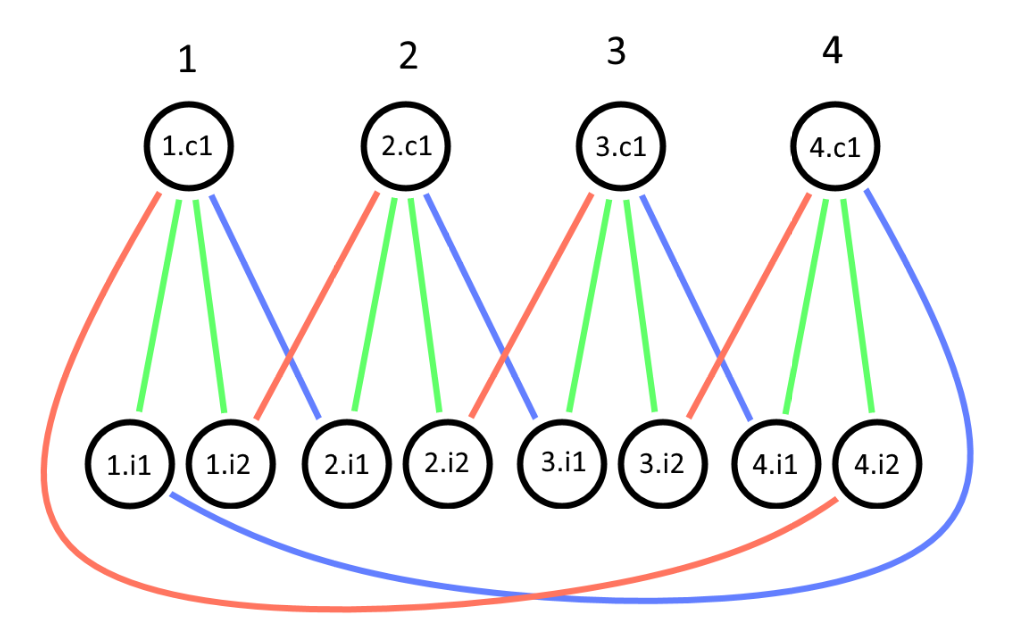
\includegraphics[scale=0.4]{Fig_1.png}
    \caption{ Метаграф с весами дуг +1, 0, 0, -1.. }
    \label{image:3.g}
\end{figure}

\textbf{Теорема 1.}

% \begin{theorem}

% Переписать исходя из того, что начальная и конечная вершины даны в определении. И того, что начальные и конечные вершины пути можно посчитать точно
% Или попробовать объединить с следующей теоремой
% Если разделить получается, что это теорема про начальную веришну пути, а следующая -- про конечную

Пусть $\eta = (e_1, ..., e_d)$ ~--- путь на метаграфе $G$, тогда на графе $G^{(r)}$ есть $r$ попарно не пересекающихся путей вида $\mu_1 ... \mu_r$ вида $\mu_j = (e'_1, ..., e'_d)$, таких что $e'_i \in R^{(r)}_{e_i}$.

\textbf{Доказательство.}

% Skorokhodov V.A. Generalization of the Reachability Problem on Directed Graphs/ Mathematics and Statistics, Vol. 8, No. 6, pp. 699 - 704, 2020. DOI: 10.13189/ms.2020.080610

Следует из определения расширения метаграфа.

\qed

\textbf{Определение 8.}

Будем говорить, что путям $\mu_j$ на графе $G^{(r)}$ соответствует путь $\eta$ на метаграфе $G$ и наоборот.

\textbf{Замечание 2.}

Из того, что некоторый путь на метаграфе $G$ является циклом не следует, что соответствующие ему пути на $G^{(r)}$ являются циклами.

% Пример

\textbf{Определение 7.}

Пусть $G = \langle V, E, w \rangle$ ~--- метаграф.

Характеристикой пути $\eta = (e_1, ..., e_d)$ будем называть

\[
    ch(\eta) = \sum_{i = 1}^d \chi_{\eta}(e_i) w(e_i).
\]

\textbf{Теорема 2.}

Пусть  $\eta = (e_1, ..., e_d)$ ~--- это некоторый путь на метаграфе $G$, его первая вершина ~--- $x$, а последняя ~--- $y$. И пусть один из соответствубщих ему путей на расширенном графе это $\mu = (e'_1, ..., e'_d)$.

Если первая вершина в пути $\mu$ ~--- $x^{(j)}$, то последняя вершина этого пути ~--- $y^{(j + ch(\eta)\mod{r})}$.

\textbf{Доказательство.}

% Как-то лучше мы это переписывали, а то просто месиво символов получается. Может там чуть ли не на "очевидно" можно было заменить

Доказательство проведём по индукции по длине пути $\eta$.

Пусть $|\eta| = 1$ и  $\eta = (e) = ((a,b))$, и $ch(\eta) = w(e)$. Дуге $e$ на метаграфе соответствуют дуги $R^{(r)}_e = \{ (a^{(j)}, b^{(j + w(e) (\mod{r}))} ) | j = 1, ..., r \}$
на расширенном графе. Таким образом, конечная вершина каждого пути $\mu_j$ ~--- $b^{(j + ch(\eta) (\mod{r}))}$.

Пусть предположение теоремы верно для всех путей короче $d$.

Пусть $|\eta| = d$ и $\eta = (e_1, ..., e_d)$.

Рассмотрим путь $\epsilon = (e_1, ..., e_{d-1})$. Пусть его последняя вершина ~--- $c$. Тогда по предположению индукции последние вершины соответствующих ему путей равны $c^{(j + ch(\epsilon) (\mod{r}))}$.

Тогда последние вершины путей, соответствующих $\eta$ будут равны $c^{(j + ch(\epsilon) + (-1)^d w(e_d) (\mod{r}))} = c^{(j + ch(\eta) (\mod{r}))}$.

\qed

Очень важными следствиями из Теоремы 2 являются две следующих теоремы.

\textbf{Теорема 3.} \textsl{(О циклах)}

Пусть $\eta$ ~--- цикл на метаграфе. Тогда соответствующие ему пути на расширенном графе являются циклами тогда и только тогда, когда $ch(\eta) = 0 (\mod{r})$.

\textbf{Теорема 4.} \textsl{(О <<крыльях>> цикла)}

Пусть $\eta = (e_1, ..., e_d)$ и $\mu = (\epsilon_1, ..., \epsilon_{\delta})$ ~--- различные пути на метаграфе с начальной вершиной $a$, конечной вершиной $b$ и $ch(\eta) = \ch(\mu) (\mod{r})$. Тогда путь на расширении, соответствующий склейке этих путей $\gamma = (e_1, \dots, e_d, \epsilon_{\delta}, \dots, \epsilon_1)$, является циклом.

Эти теоремы дают метод нахождения циклов на расширенном графе, описываемый следующим алгоритмом:

\textbf{Алгоритм 1.}

% Мне кажетс, что этот алгоритм можно переписать крафсивее
% Доказательство тут, кажется, встроено в само определение алгоритма

Поиска цикла с длинной меньше или раной заданному числу $l \in \mathbb{N}$.

Пусть $G = \langle A \cup B, E,w\rangle$ ~--- метаграф. Для каждой вершины $a \in A:$

\begin{itemize}
    \item Пометим $a$ парой $(0, 0)$.
    \item В цикле по поколениям $g$ от $1$ до $l$:
      \begin{itemize}
      \item Для всех меток $label = (ch, g - 1)$:
        \begin{itemize}
        \item Вершину, которая помечена меткой $label$, обозначим $v$.
        \item Для всех дуг $e: v \in f(e)$:
          \begin{itemize}
          \item $ch' = ch + (-1)^{g} w(e)$
          \item Обозначим $v'$ вершину, такую, что $v' \in f(e), v' \neq v$.
          \item Если $v'$ ещё не была помечена меткой $(ch', g') \forall g'$ ~--- пометим её парой $(ch', g)$.
          \item Если $v'$ помечена помечена парой $(ch', g)$ ~--- сообщаем о том, что найден цикл длины $g * 2$ и завершаем работу алгоритма.
          \end{itemize}
        \end{itemize}
      \end{itemize}
    \item Сообщаем о том, что цикл не найден и завершаем работу алгоритма.
\end{itemize}

$/*$ Надо добавить пример, сейчас он есть только на бумажечке $*/$

\pagebreak
\section*{Построение графов с заданным обхватом}

Пусть $G = \langle V, E, w \rangle$ ~--- метаграф, причём $V = A \cup B$ и $w(e_i) = x_i \forall i = 0..|E|$.

Для каждой пары вершин $a$ и $v$, таких что $a \in A$ и $v \in V$, рассмотрим все неравенства вида $ch(\eta) \neq ch(\mu)$ Где $\eta$ и $\mu$ ~--- различные пути из $a$ в $v$, одинаковой длины не большей некоторого заданного значения $l \in N$.

Систему, содержащую все такие неравенств представим в виде (1).

\begin{equation}
    \centering
    \left\{
        \begin{array}{ll}
            a_{1,1} x_1 + ... + a_{1,e} x_e + b &\neq 0\\
            ...\\
            a_{l,1} x_1 + ... + a_{l,1} x_e + b &\neq 0\\
        \end{array}
    \right.
    \label{eqs:example}
\end{equation}

Пусть $G$ ~--- некоторый метаграф. Тогда справедлива следующая теорема.

\textbf{Теорема 5.}

Для $G$ существует расширение с обхватом большим $2l$  тогда и только тогда, когда система неравенств (1) для графа $G$ совместна.

\textbf{Доказательство.}

Из теоремы 4 следует, что характеристики путей, начинающихся и заканчивающихся в одной вершине равны, тогда и только тогда, когда они образуют цикл. Следовательно, при построении системы (1) ичерпываются все пары путей, которые могли бы образовать цикл. Таким образом существование решения системы (1) эквивалентно существованию расширения с обхватом большим, чем удвоенная длина максимального пути.

\qed

Для построения системы вида (\ref{eqs:example}) для заданного метаграфа $G$ можно воспользоваться следующим алгоритмом, являющимся модификацией Алгоритма 1.

\textbf{Алгоритм 2.}

% Аналогично предыдущему алгоритму, надо бы переписать красивее. Может вообще удалить, сказав, мол, "просто пишем x вместо чисел", не уверен

Пусть $G = \langle A \cup B, E,w\rangle$ ~--- метаграф причём $w(e_i) = x_i \forall i = 0..|E|$. Для каждой вершины $a \in A:$

\begin{itemize}
    \item Пометим $a$ парой $(0, 0)$.
    \item В цикле по поколениям $g$ от $1$ до $l$:
      \begin{itemize}
      \item Для всех меток $label = (ch, g - 1)$:
        \begin{itemize}
        \item Вершину, которая помечена меткой $label$, обозначим $v$.
        \item Для всех дуг $e: v \in f(e)$:
          \begin{itemize}
          \item $ch' = ch + (-1)^{g} w(e)$
          \item Обозначим $v'$ вершину, такую, что $v' \in f(e), v' \neq v$.
          \item Если $v'$ ещё не была помечена меткой $(ch', g') \forall g'$ ~--- пометим её парой $(ch', g)$.
          \end{itemize}
        \end{itemize}
      \end{itemize}
    \item Возвращаем систему, содержащую все неравенства вида, $ch_1 \neq \ch_2$ для всех пар меток на одной и той же вершине с одним и тем же поколением.
\end{itemize}

$/*$ Пример $*/$

\section*{Решение систем не равенств}

Поиск минимального решения для систем неравенств вида (\ref{eqs:example}), представленных в прошлой главе представляется вычислительно трудной задачей. Она предполагает перебор всех возможных решений с выбором минимального. Однако некоторое решение можно найти, воспользовавшись следующим алгоритмом.

\textbf{Алгоритм 3.}

\begin{enumerate}
    \item $e$ ~--- количество неизвестных в системе неравенств.
    \item Если в системе содержится неравенство вида $0 \neq 0$, то система не имеет решений, алгоритм завершается, сообщая, что решений нет.
    \item Найдём все неравенства вида $a x_e + b \neq 0$. Обозначим множество таких неравенств $I$.
    \item Выберем число $v$ такое, что $v \neq -b/a \forall a x_e + b \in I$, если $I = \varnothing$, то положим $v = 0$. Такое число можно найти, так как неравенств конечное количество. В результате этой замены не возникнет неравенства вида $0 \neq 0$ по условию выбора $v$.
    \item Заменим во всех неравенствах $x_e$ на $v$ и добавим в решение элемент $x_e = v$.
    \item Если $e = 1$ ~--- завершим работу алгоритма.
    \item Положим $e = e - 1$ переменной и вернёмся на шаг 3.
\end{enumerate}

$/*$ Пример $*/$

\textbf{Замечание.}

Результатом работы алгоритма поиска рещшения системы неравенств не обязательно будет минимальное решение.

% Пример

\section*{Оценка работы алгоритма}

Описанный выше алгоритм построения графов с заданным обхватом не обязательно порождает решения с минимальным количеством вершин.

% Пример?

С увеличением требуемого обхвата количество вершин у результирующего графа растёт очень быстро.

Для метаграфа $G = \langle V,E,w \rangle$, количество вершин можно оценить снизу числом $  $ % Надо вспомнить, каким числом мы его оценивали

\textbf{Доказательство.}

% Оценки сверху мы, кажется, никакой не давали

% три пути, смотреть скриншот

\end{document}